\newpage
\section{Arhitektura sistema}
\subsection{Osnovni prikaz}
Sledi prikaz karakteristika arhitekture informacionog sistema za poručivanje hrane jednog restorana. Odluke su donošene u skladu sa prirodom i funkcionalnim zahtevima sistema, kao i potrebama korisnika i razvijaoca.Time su određene sledeće karakteristike arhitekture informacionog sistema:
\begin{enumerate}
    \item Tip aplikacije: Veb aplikacija
    \item Strategije isporučivanje: jedan serverski i više klijentskih računara
    \item Odgovarajuće tehnologije: HTML5, MYSQL, JS, CSS, BOOTSTRAP
    \item Prateće komponente:
    \begin{enumerate}
        \item \textbf{Logovanje na sistem:} Podsistem za autentikaciju korisnika. Sadrži GUI komponentu za učitavanje klijentskih podataka i komponentu za validaciju podataka.
        \item \textbf{Backup baze:} Predstavlja podsistem za pravljenje kopija baze. Uz to, vodi računa o konzistentnosti kopija, intervalu backup-ovanja i sl.
        \item \textbf{Pomoć:} Sadrži uputstvo za upotrebu, kontakt i podršku.
        
    \end{enumerate}
\end{enumerate}

\subsection{Tip arhitekture i slojevi}
Arhitektura sistema je osmišljena kao klijent-server tip arhitekture čiji su entiteti bazirani na tri (odnosno četiri) sloja.
\begin{enumerate}
    \item \textbf{Model} sadrži skup klasa koje opisuju sve entitete iz informacionog sistema. Model se sastoji od sledećih klasa sa opisanom funkcijom:
    \begin{itemize}
        \item \emph{Korisnik} je klasa koja sadrži sve lične informacije o korisniku aplikacije. Njegova polja su identična kolonama u tabeli Osoba (slika \ref{fig:slika_baza}), takođe sadrži i alternativne adrese koje jedan korisnik može imati.
        \item \emph{Zaposleni} je klasa koja sadrži sve lične informacije o zaposlenom u restoranu. Polja klase Zaposleni identična su kolonama u tabeli Osoba (slika \ref{fig:slika_baza}), takođe sadrži i informacije o njegovoj ulozi o sistemu, broj broj preostalih/iskorišćenih slobodnih dana, kao i podatak da li je taj zaposleni trenutno na odmoru.
        \item \emph{ZahtevZaOdsustvom} je klasa koja sadrži sva polja istoimenog entiteta. U ovoj klasi, nalaze se sve potrebne informacije za obradu zahteva zaposlenog za odlazak na plaćeno/neplaćeno odsustvo kao što su datum\_početka i datum\_završetka, kao i informacija o tome da li je određeni zahtev prihvaćen ili odbijen.
        \item \emph{Namirnica} je klasa oja sadrži podatke o svakoj namirnici koja se trenutno nalazi u magacinu. Ona direktno oslikava entitet Namirnice koji se nalazi u bazi.
         \item \emph{Jelo} je klasa koja oslikava prikaz jednog jela u jelovniku koji se prikazuje korisniku.
         \item \emph {Priprema} je klasa koja sadrži id-jeve klase Jelo i klase Namirnice i predstavlja njihovu agregaciju. Pruža nam informaciju o tome koje namirnice ulaze u sastav jednog jela.
         \item \emph{Porudžbina} je klasa koja sadrži sve informacije koje se prosleđuju nakon što korisnik uputi zahtev za poručivanjem određenog jela. Sadrži informacije o korisniku koji prosleđuje zahtev tj. id korisnika i propratne opisne informacije za datu porudžbinu.
         \item \emph{Spisak} je klasa koja sadrži id objekta klase Porudžbina, kao i listu id-jeva objekata klase Jelo. Informacije iz ove klase nam pomažu da vidimo koja sve jela ulaze u sastav jedne određene porudžbine, koja je njihova količina, kao i to da li je određeno jelo trenutno spremljeno ili se na njega čeka.
         \item \emph{Dostava} je klasa koja sadrži id porudžbine sa kojom je data dostava povezana, id zaposlenog koji će da izvrši dostavu. Beleže se i informacije o tome da li je određena dostava uspešno obavljena i koliko je vremena trebalo dostavljaču da izvrši dostavu. 
         \item \emph{Ocena} je klasa koja se koristi za operisanje ocenama odnosno recenzijama korisnika na određeno jelo. Svaki korisnik koji je naručio neko jelo u nekoj od njegovih prethodnih porudžbina, ima mogućnost da ostavi recenziju, odnosno da ostavi komentar uz datu ocenu (polje \emph{vrednost}). Ovaj deo modela nam koristi za praćenje korisničkih iskustava prilikom poručivanja određenog jela.
    \end{itemize}
    \item \textbf{View} odnosno pogled prikazuje podatke iz modela, u formatu pogodnom za interakciju, kao komponentu korisničkog interfejsa. Za svaki slučaj upotrebe kreiran je jedan view. U zavisnosti od toga da li je osoba koja poseduje nalog zaposleni u restoranu ili korisnik koji poručuje hranu, prikazuju im se različiti interfejsi nakon logovanja na sistem. 
    \begin{itemize} 
    \item Prvi i osnovni deo View-a je početna strana. Na početnoj strani korisnik/zaposleni može da se prijavi ili da napravi novi nalog ukoliko ga ne poseduje. Prilikom registracije korisniku se prikazuje stranica sa poljima koje je neophodno da popuni kako bi uspešno kreirao nalog. Kod kreiranja naloga zaposlenog postoji jedna razlika. Nalog za zaposlene kreira menadžer, a ne zaposleni lično. Pri ovom kreiranju, pored osnovnih informacija, menadžer unosi i funkciju novozaposlenog u sistemu. Ovo se nalazi na kartici pod nazivom \emph{Nalozi}. Karticu \emph{Nalog} imaju i korisnik i zaposleni. Ovde se nalaze sve njihove lične informacije koje su uneli tokom registracije, od kojih određene mogu da ažuriraju, uklone ili dodaju.
    \item \emph{Utisci} predstavljaju još jedan deo korisničkog interfejsa kome korisnik može da pristupi. Na ovoj kartici korisnik može da unese komentar, naziv jela za koji ostavlja utisak i ocenu koju daje.
    \item \emph Korisnik može i, nakon što se ulogovao na sistem, da pristupi i istoriji svojih porudžbina otvaranjem kartice \emph{Moje porudžbine}. Tu može da vidi detalje o svim svojim prethodno poručivanim jelima.
    \item Kada korisnik poželi da napravi novu porudžbinu, on odlazi na karticu \emph{Poručivanje} gde mu se prikazuje jelovnik i tada ima mogućnost da odabere jelo i obavi porudžbinu.
    
    \item \emph{Upravljanje porudžbinama} je deo UI-ja koji se prikazuje isključivo koordinatoru. Na ovoj kartici koordinator je u mogućnosti da vidi porudžbine tj. sve detalje vezane za određene porudžbine i da ih prihvati ili odbije, tačnije, ovde se vrši obrada i pregled porudžbina.
    
    \item Kartica pod nazivom \emph{Raspoloživost namirnica} prikazuje se koordinatoru. Njemu je ovde omogućen pregled količine svih namirnica u magacinu u svrhu prihvatanja/odbijanja porudžbine. Deo interfejsa koji je specifičan isključivo za magacionera, a odnosi se na namirnice su kartice \emph{Stanje magacina} , na kojoj on može da vidi stanje preostalih namirnica u magacinu i da poruči namirnice koje nedostaju, i \emph{Naručene namirnice}, gde magacioner može da vidi šta je od namirnica naručio i kasnije, kada pristignu, da to evidentira.
    
    
    \item Deo interfejsa koji se tiče obrade i pregleda odmora zaposlenom koji želi da zatraži odsustvo prikazuje se u kartici \emph{Odmor}. Tu zaposleni može da kreira novi zahtev za odmorom, kao i da proveri u kakvom su stanju njegovi prethodno zatraženi zahtevi.
    Menadžeru je na raspolaganju i kartica pod nazivom \emph{Zahtevi Zaposlenih} gde ima pregled stanja njihovih dana odsustva i broja raspoloživih slobodnih dana za svakog zaposlenog. Takođe, ovde menadžer obrađuje zahteve zaposlenih, prihvata ih ili ih odbija.
    \end{itemize}
    \item \textbf{Kontroler} sadrži pripremu podataka za pogled, proračune, kao i njihovu pripremu pre slanja na obradu modelu. On je u ovom slučaju izdeljen na dve komponente - klijent, odnosno server kontroler. Klijentska strana obavlja komunikaciju između pogleda i modela u zavisnosti od korisnikovog unosa, dok se na serverskoj instanci obavlja autentikacija, autorizacija, i upravljanje podacima.
\end{enumerate}

\begin{figure}[!ht]
    \leavevmode
    \centering
    \advance\leftskip-1.3cm
    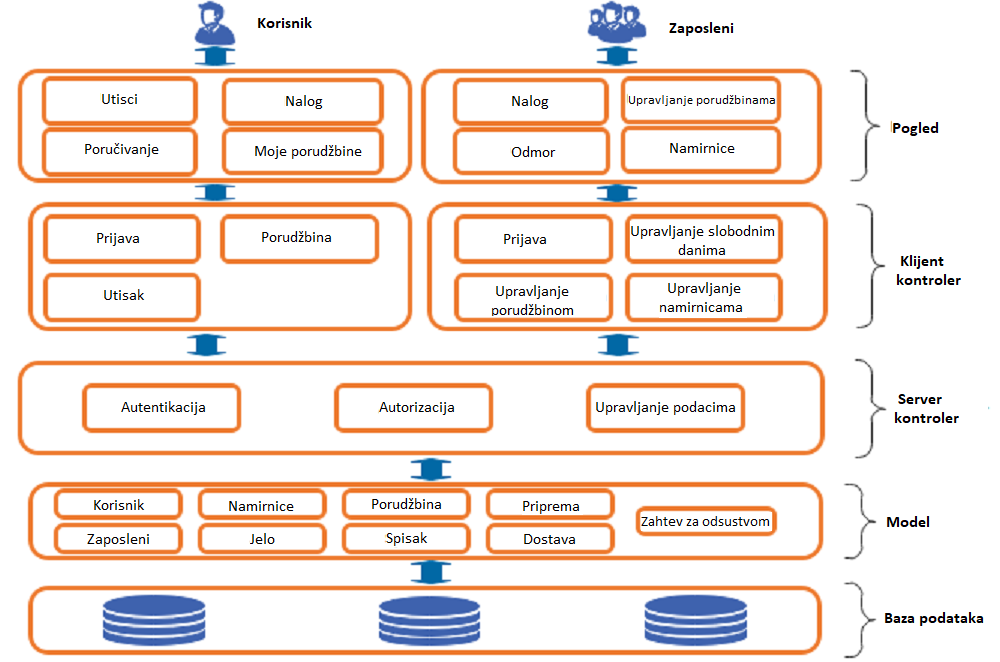
\includegraphics[width=1.2\textwidth]{slike/arh1.png}
    \caption{Arhitektura sistema}
    \label{fig:slika11}
\end{figure}
\leavevmode
